\documentclass{article}
%\documentclass[journal]{IEEEtran}
%\documentclass{report}
%\documentclass{acta}

\usepackage{graphicx}

\begin{document}

\title{Efficient Policy Enforcement in Android Applications with Counterexample-Guided Abstraction Refinement}
\author{Yu Feng}

\maketitle

\begin{abstract}
Previously, we presented Apposcopy, a new semantics-based approach 
for identifying a prevalent class of Android malware that steals 
private user information. However, in practice, we also noticed 
that several malicious behaviors can only be triggered under a 
certain sequential system events. To detect such behaviors and make
an enhancement on our current system, one way is to perform model
checking on the abstract state machine of a given application.
But the downside is that the system will take a long time to analyze
a single application. 

To detect malware that violate the security policy specified by users 
in terms of temporal formulas in a efficient way, we apply 
counterexample-guided abstraction refinement-based(CEGAR) model 
checking. The intuition is, we build the TICCG(Temporal Inter-Component 
communication Call Graph) which is the abstract state machine of a given 
Android applicaton, then the system will check the validity of the application
with respect to a set of temporal properties. If it's valid, then 
our system satisfies current properties. If it's invalid, it could
be (1) a true violation, which we report it to the user; Or (2)
a false positive. In this case, we will refine the TICCG based on
the counterexample generated by the trace of system events.
\end{abstract}


\section{Introduction}
As  the most popular mobile operating system, the Android platform 
is a growing target for  mobile malware~\cite{usreport}.
Today, many of the malicious applications that afflict  Android users  exploit
the private and monetized information
stored in a user's smartphone. % such as the user's contacts, photos, or
%account information. 

To mitigate the above problems, researchers have been working on either 
static analysis-based techniques, such as semantic-based approaches and taint analysis, 
or dynamic analysis based on monitoring the execution traces of a 
given application. However, there are still corpus of malware that is hard to detect 
by existing technique. According to a recent literature~\cite{pegasus}, there are
several sophisticated Android malware and their malcious behaviors can only 
be triggered under a specific event sequences.

In response to the  rapid dissemination of 
Android malware, there is  a real need for tools that can automatically
detect malicious applications that violate a set of safty properties 
specified by an auditor.

\subsection{Challenges}
To the best of our knowledge, there is no previous model checking tools for 
Android applications which can scale in large applications.
Pegasus\cite{pegasus} models Android applications as "Permission Event Graph"
and checking the safty properties encoded by Java program. While it can 
differentiate benign applicaton and malicious application through a set 
of safty properties, it also suffers the performance issue: Most of the 
applications will take more than 1000 seconds to terminate. 

JAM\cite{cegar12} introduced CEGAR to reduce the runtime overhead of web 
application in the context of Javascript, which is closed
to our current work.

\section{Overview}
\label{sec:overview}

% Figure
\begin{figure}
\centerline{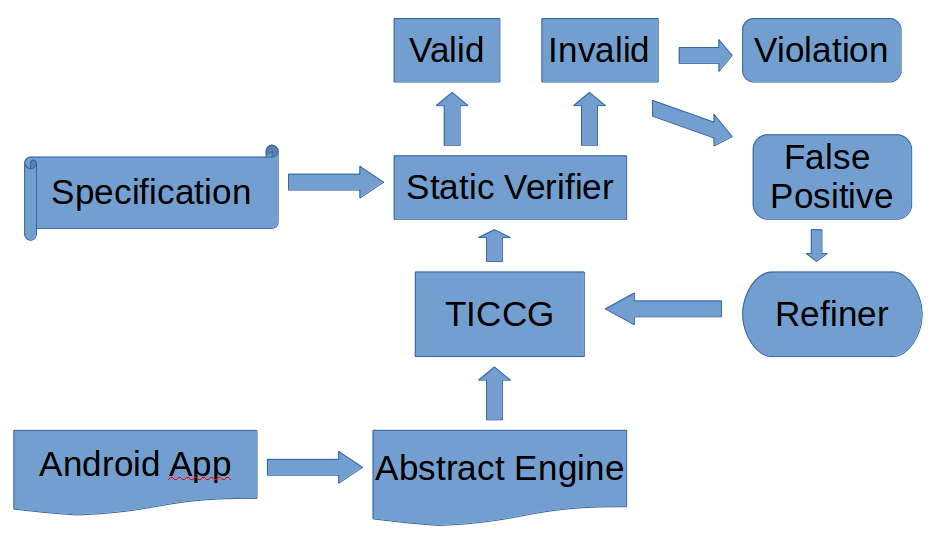
\includegraphics[scale=0.4]{sysgraph}}
\caption{System Overview}
\label{fig:one}
\end{figure}

Figure~\ref{fig:one} shows an overview of the system architecture.
It takes as input an Android application(source code or bytecode) 
and a set of temporal properties encoded as datalog. By running the 
abstract engine, the system first converts the Android application 
to TICCG(Temporal Inter-Component Communication Call Graph), 
which is the augmented version of our previous work\cite{apposcopy}
by modeling the system events and system APIs in the graph. 
Then the static verifier will perform stardard model checking to 
verify whether all the temporal properties are valid with respect 
to a given TICCG. If the result is valid and since our analysis is 
sound, we conclude that current application will not violate those
temporal properties. If the result is invalid, then there exists two
cases: (1) We detect a true violation and report it to the user; 
(2) It is a false positive because our analysis is imprecise or the 
given temporal formulas are too strong to exclude some benign applications.
For the first case, we will use current system event traces as a counterexample
\cite{clarkecegar} and  run the refiner to refine the original 
TICCG to prune the search space; For the second case, we can manully
modify the temporal formulas based on some domain specific information.


\subsection{Contributions}
The main contributions of this work can be summarized as follows.
% itemize
\begin{itemize}
\item We apply model checking to verify whether a given applicatino violates
a set of pre-defined safty policies and make it scale in real world 
applications;
\item We come up with TICCG, a new abstraction for Android application
that models the temporal behaviors of system APIs and system events;
\item We apply the counterexample-guided abstraction refinement-based(CEGAR) 
technique in Android application and use it to improve the performance 
of the system dramatically.
\end{itemize}



\section{Conclusion}

Lorem ipsum dolor sit amet, consectetur adipisicing elit, sed do eiusmod tempor
incididunt ut labore et dolore magna aliqua. Ut enim ad minim veniam, quis
nostrud exercitation ullamco laboris nisi ut aliquip ex ea commodo consequat.
Duis aute irure dolor in reprehenderit in voluptate velit esse cillum dolore eu
fugiat nulla pariatur.
% Bibliography
%\bibliographystyle{ACM-Reference-Format-Journals}
%\bibliography{mybib}
 

\end{document}
